\documentclass[1p]{elsarticle_modified}
%\bibliographystyle{elsarticle-num}

%\usepackage[colorlinks]{hyperref}
%\usepackage{abbrmath_seonhwa} %\Abb, \Ascr, \Acal ,\Abf, \Afrak
\usepackage{amsfonts}
\usepackage{amssymb}
\usepackage{amsmath}
\usepackage{amsthm}
\usepackage{scalefnt}
\usepackage{amsbsy}
\usepackage{kotex}
\usepackage{caption}
\usepackage{subfig}
\usepackage{color}
\usepackage{graphicx}
\usepackage{xcolor} %% white, black, red, green, blue, cyan, magenta, yellow
\usepackage{float}
\usepackage{setspace}
\usepackage{hyperref}

\usepackage{tikz}
\usetikzlibrary{arrows}

\usepackage{multirow}
\usepackage{array} % fixed length table
\usepackage{hhline}

%%%%%%%%%%%%%%%%%%%%%
\makeatletter
\renewcommand*\env@matrix[1][\arraystretch]{%
	\edef\arraystretch{#1}%
	\hskip -\arraycolsep
	\let\@ifnextchar\new@ifnextchar
	\array{*\c@MaxMatrixCols c}}
\makeatother %https://tex.stackexchange.com/questions/14071/how-can-i-increase-the-line-spacing-in-a-matrix
%%%%%%%%%%%%%%%

\usepackage[normalem]{ulem}

\newcommand{\msout}[1]{\ifmmode\text{\sout{\ensuremath{#1}}}\else\sout{#1}\fi}
%SOURCE: \msout is \stkout macro in https://tex.stackexchange.com/questions/20609/strikeout-in-math-mode

\newcommand{\cancel}[1]{
	\ifmmode
	{\color{red}\msout{#1}}
	\else
	{\color{red}\sout{#1}}
	\fi
}

\newcommand{\add}[1]{
	{\color{blue}\uwave{#1}}
}

\newcommand{\replace}[2]{
	\ifmmode
	{\color{red}\msout{#1}}{\color{blue}\uwave{#2}}
	\else
	{\color{red}\sout{#1}}{\color{blue}\uwave{#2}}
	\fi
}

\newcommand{\Sol}{\mathcal{S}} %segment
\newcommand{\D}{D} %diagram
\newcommand{\A}{\mathcal{A}} %arc


%%%%%%%%%%%%%%%%%%%%%%%%%%%%%5 test

\def\sl{\operatorname{\textup{SL}}(2,\Cbb)}
\def\psl{\operatorname{\textup{PSL}}(2,\Cbb)}
\def\quan{\mkern 1mu \triangleright \mkern 1mu}

\theoremstyle{definition}
\newtheorem{thm}{Theorem}[section]
\newtheorem{prop}[thm]{Proposition}
\newtheorem{lem}[thm]{Lemma}
\newtheorem{ques}[thm]{Question}
\newtheorem{cor}[thm]{Corollary}
\newtheorem{defn}[thm]{Definition}
\newtheorem{exam}[thm]{Example}
\newtheorem{rmk}[thm]{Remark}
\newtheorem{alg}[thm]{Algorithm}

\newcommand{\I}{\sqrt{-1}}
\begin{document}

%\begin{frontmatter}
%
%\title{Boundary parabolic representations of knots up to 8 crossings}
%
%%% Group authors per affiliation:
%\author{Yunhi Cho} 
%\address{Department of Mathematics, University of Seoul, Seoul, Korea}
%\ead{yhcho@uos.ac.kr}
%
%
%\author{Seonhwa Kim} %\fnref{s_kim}}
%\address{Center for Geometry and Physics, Institute for Basic Science, Pohang, 37673, Korea}
%\ead{ryeona17@ibs.re.kr}
%
%\author{Hyuk Kim}
%\address{Department of Mathematical Sciences, Seoul National University, Seoul 08826, Korea}
%\ead{hyukkim@snu.ac.kr}
%
%\author{Seokbeom Yoon}
%\address{Department of Mathematical Sciences, Seoul National University, Seoul, 08826,  Korea}
%\ead{sbyoon15@snu.ac.kr}
%
%\begin{abstract}
%We find all boundary parabolic representation of knots up to 8 crossings.
%
%\end{abstract}
%\begin{keyword}
%    \MSC[2010] 57M25 
%\end{keyword}
%
%\end{frontmatter}

%\linenumbers
%\tableofcontents
%
\newcommand\colored[1]{\textcolor{white}{\rule[-0.35ex]{0.8em}{1.4ex}}\kern-0.8em\color{red} #1}%
%\newcommand\colored[1]{\textcolor{white}{ #1}\kern-2.17ex	\textcolor{white}{ #1}\kern-1.81ex	\textcolor{white}{ #1}\kern-2.15ex\color{red}#1	}

{\Large $\underline{11a_{3}~(K11a_{3})}$}

\setlength{\tabcolsep}{10pt}
\renewcommand{\arraystretch}{1.6}
\vspace{1cm}\begin{tabular}{m{100pt}>{\centering\arraybackslash}m{274pt}}
\multirow{5}{120pt}{
	\centering
	\includegraphics[width=112pt]{../../../GIT/diagram.site/Diagrams/png/252_11a_3.png}\\
\ \ \ A knot diagram\footnotemark}&
\allowdisplaybreaks
\textbf{Linearized knot diagam} \\
\cline{2-2}
 &
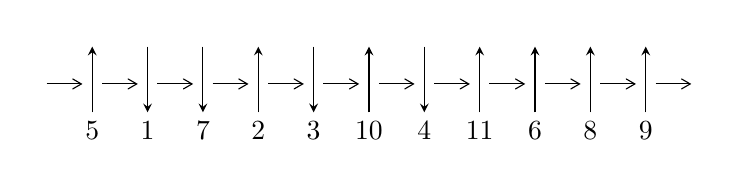
\begin{tikzpicture}[x=20pt, y=17pt]
	% nodes
	\node (C0) at (0, 0) {};
	\node (C1) at (1, 0) {};
	\node (C1U) at (1, +1) {};
	\node (C1D) at (1, -1) {5};

	\node (C2) at (2, 0) {};
	\node (C2U) at (2, +1) {};
	\node (C2D) at (2, -1) {1};

	\node (C3) at (3, 0) {};
	\node (C3U) at (3, +1) {};
	\node (C3D) at (3, -1) {7};

	\node (C4) at (4, 0) {};
	\node (C4U) at (4, +1) {};
	\node (C4D) at (4, -1) {2};

	\node (C5) at (5, 0) {};
	\node (C5U) at (5, +1) {};
	\node (C5D) at (5, -1) {3};

	\node (C6) at (6, 0) {};
	\node (C6U) at (6, +1) {};
	\node (C6D) at (6, -1) {10};

	\node (C7) at (7, 0) {};
	\node (C7U) at (7, +1) {};
	\node (C7D) at (7, -1) {4};

	\node (C8) at (8, 0) {};
	\node (C8U) at (8, +1) {};
	\node (C8D) at (8, -1) {11};

	\node (C9) at (9, 0) {};
	\node (C9U) at (9, +1) {};
	\node (C9D) at (9, -1) {6};

	\node (C10) at (10, 0) {};
	\node (C10U) at (10, +1) {};
	\node (C10D) at (10, -1) {8};

	\node (C11) at (11, 0) {};
	\node (C11U) at (11, +1) {};
	\node (C11D) at (11, -1) {9};
	\node (C12) at (12, 0) {};

	% arrows
	\draw[->,>={angle 60}]
	(C0) edge (C1) (C1) edge (C2) (C2) edge (C3) (C3) edge (C4) (C4) edge (C5) (C5) edge (C6) (C6) edge (C7) (C7) edge (C8) (C8) edge (C9) (C9) edge (C10) (C10) edge (C11) (C11) edge (C12) ;	\draw[->,>=stealth]
	(C1D) edge (C1U) (C2U) edge (C2D) (C3U) edge (C3D) (C4D) edge (C4U) (C5U) edge (C5D) (C6D) edge (C6U) (C7U) edge (C7D) (C8D) edge (C8U) (C9D) edge (C9U) (C10D) edge (C10U) (C11D) edge (C11U) ;
	\end{tikzpicture} \\
\hhline{~~} \\& 
\textbf{Solving Sequence} \\ \cline{2-2} 
 &
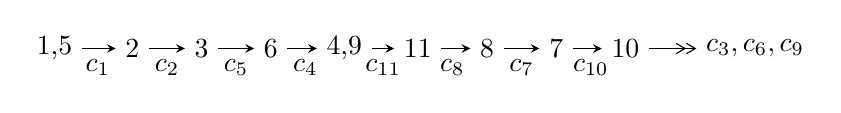
\begin{tikzpicture}[x=25pt, y=7pt]
	% node
	\node (A0) at (-1/8, 0) {1,5};
	\node (A1) at (1, 0) {2};
	\node (A2) at (2, 0) {3};
	\node (A3) at (3, 0) {6};
	\node (A4) at (65/16, 0) {4,9};
	\node (A5) at (41/8, 0) {11};
	\node (A6) at (49/8, 0) {8};
	\node (A7) at (57/8, 0) {7};
	\node (A8) at (65/8, 0) {10};
	\node (C1) at (1/2, -1) {$c_{1}$};
	\node (C2) at (3/2, -1) {$c_{2}$};
	\node (C3) at (5/2, -1) {$c_{5}$};
	\node (C4) at (7/2, -1) {$c_{4}$};
	\node (C5) at (37/8, -1) {$c_{11}$};
	\node (C6) at (45/8, -1) {$c_{8}$};
	\node (C7) at (53/8, -1) {$c_{7}$};
	\node (C8) at (61/8, -1) {$c_{10}$};
	\node (A9) at (10, 0) {$c_{3},c_{6},c_{9}$};

	% edge
	\draw[->,>=stealth]	
	(A0) edge (A1) (A1) edge (A2) (A2) edge (A3) (A3) edge (A4) (A4) edge (A5) (A5) edge (A6) (A6) edge (A7) (A7) edge (A8) ;
	\draw[->>,>={angle 60}]	
	(A8) edge (A9);
\end{tikzpicture} \\ 

\end{tabular} \\

\footnotetext{
The image of knot diagram is generated by the software ``\textbf{Draw programme}" developed by Andrew Bartholomew(\url{http://www.layer8.co.uk/maths/draw/index.htm\#Running-draw}), where we modified some parts for our purpose(\url{https://github.com/CATsTAILs/LinksPainter}).
}\phantom \\ \newline 
\centering \textbf{Ideals for irreducible components\footnotemark of $X_{\text{par}}$} 
 
\begin{align*}
I^u_{1}&=\langle 
4.73407\times10^{19} u^{65}-1.78062\times10^{20} u^{64}+\cdots+6.92121\times10^{19} b-9.60242\times10^{19},\\
\phantom{I^u_{1}}&\phantom{= \langle  }2.00992\times10^{19} u^{65}-1.27810\times10^{20} u^{64}+\cdots+6.92121\times10^{19} a+5.30233\times10^{20},\;u^{66}-4 u^{65}+\cdots-14 u+1\rangle \\
I^u_{2}&=\langle 
b-1,\;u^4- u^3+2 u^2+a- u+1,\;u^5- u^4+2 u^3- u^2+u-1\rangle \\
I^u_{3}&=\langle 
- a u+b+u,\;a^2- a u-3 a+2,\;u^2+u+1\rangle \\
\\
\end{align*}
\raggedright * 3 irreducible components of $\dim_{\mathbb{C}}=0$, with total 75 representations.\\
\footnotetext{All coefficients of polynomials are rational numbers. But the coefficients are sometimes approximated in decimal forms when there is not enough margin.}
\newpage
\renewcommand{\arraystretch}{1}
\centering \section*{I. $I^u_{1}= \langle 4.73\times10^{19} u^{65}-1.78\times10^{20} u^{64}+\cdots+6.92\times10^{19} b-9.60\times10^{19},\;2.01\times10^{19} u^{65}-1.28\times10^{20} u^{64}+\cdots+6.92\times10^{19} a+5.30\times10^{20},\;u^{66}-4 u^{65}+\cdots-14 u+1 \rangle$}
\flushleft \textbf{(i) Arc colorings}\\
\begin{tabular}{m{7pt} m{180pt} m{7pt} m{180pt} }
\flushright $a_{1}=$&$\begin{pmatrix}1\\0\end{pmatrix}$ \\
\flushright $a_{5}=$&$\begin{pmatrix}0\\u\end{pmatrix}$ \\
\flushright $a_{2}=$&$\begin{pmatrix}1\\- u^2\end{pmatrix}$ \\
\flushright $a_{3}=$&$\begin{pmatrix}u^2+1\\- u^2\end{pmatrix}$ \\
\flushright $a_{6}=$&$\begin{pmatrix}- u^5-2 u^3- u\\u^5+u^3+u\end{pmatrix}$ \\
\flushright $a_{4}=$&$\begin{pmatrix}- u\\u^3+u\end{pmatrix}$ \\
\flushright $a_{9}=$&$\begin{pmatrix}-0.290400 u^{65}+1.84665 u^{64}+\cdots+17.1503 u-7.66099\\-0.683994 u^{65}+2.57271 u^{64}+\cdots-8.88365 u+1.38739\end{pmatrix}$ \\
\flushright $a_{11}=$&$\begin{pmatrix}0.477604 u^{65}-0.313880 u^{64}+\cdots+9.01518 u-4.46864\\-1.76402 u^{65}+7.20916 u^{64}+\cdots-25.9654 u+2.45043\end{pmatrix}$ \\
\flushright $a_{8}=$&$\begin{pmatrix}0.352013 u^{65}-2.74835 u^{64}+\cdots+30.8461 u-5.72790\\1.33994 u^{65}-5.22709 u^{64}+\cdots+16.3365 u-0.873918\end{pmatrix}$ \\
\flushright $a_{7}=$&$\begin{pmatrix}0.996758 u^{65}-2.80838 u^{64}+\cdots+21.4371 u-5.07963\\-1.17865 u^{65}+4.19945 u^{64}+\cdots-8.87499 u+0.996758\end{pmatrix}$ \\
\flushright $a_{10}=$&$\begin{pmatrix}0.773579 u^{65}-2.81719 u^{64}+\cdots+35.3229 u-9.01284\\-0.443910 u^{65}+1.66335 u^{64}+\cdots-5.63834 u+1.19827\end{pmatrix}$\\ \flushright $a_{10}=$&$\begin{pmatrix}0.773579 u^{65}-2.81719 u^{64}+\cdots+35.3229 u-9.01284\\-0.443910 u^{65}+1.66335 u^{64}+\cdots-5.63834 u+1.19827\end{pmatrix}$\\&\end{tabular}
\flushleft \textbf{(ii) Obstruction class $= -1$}\\~\\
\flushleft \textbf{(iii) Cusp Shapes $= \frac{88536532098082237941}{69212056571253139646} u^{65}-\frac{346942669555547012397}{69212056571253139646} u^{64}+\cdots-\frac{2682685309410699867097}{69212056571253139646} u+\frac{417517236906079889612}{34606028285626569823}$}\\~\\
\newpage\renewcommand{\arraystretch}{1}
\flushleft \textbf{(iv) u-Polynomials at the component}\newline \\
\begin{tabular}{m{50pt}|m{274pt}}
Crossings & \hspace{64pt}u-Polynomials at each crossing \\
\hline $$\begin{aligned}c_{1},c_{4}\end{aligned}$$&$\begin{aligned}
&u^{66}+4 u^{65}+\cdots+14 u+1
\end{aligned}$\\
\hline $$\begin{aligned}c_{2}\end{aligned}$$&$\begin{aligned}
&u^{66}+32 u^{65}+\cdots-86 u+1
\end{aligned}$\\
\hline $$\begin{aligned}c_{3},c_{7}\end{aligned}$$&$\begin{aligned}
&u^{66}+2 u^{65}+\cdots-16 u-16
\end{aligned}$\\
\hline $$\begin{aligned}c_{5}\end{aligned}$$&$\begin{aligned}
&u^{66}-4 u^{65}+\cdots+4020 u+977
\end{aligned}$\\
\hline $$\begin{aligned}c_{6},c_{9}\end{aligned}$$&$\begin{aligned}
&u^{66}-3 u^{65}+\cdots-96 u+32
\end{aligned}$\\
\hline $$\begin{aligned}c_{8},c_{10},c_{11}\end{aligned}$$&$\begin{aligned}
&u^{66}+8 u^{65}+\cdots-12 u-1
\end{aligned}$\\
\hline
\end{tabular}\\~\\
\newpage\renewcommand{\arraystretch}{1}
\flushleft \textbf{(v) Riley Polynomials at the component}\newline \\
\begin{tabular}{m{50pt}|m{274pt}}
Crossings & \hspace{64pt}Riley Polynomials at each crossing \\
\hline $$\begin{aligned}c_{1},c_{4}\end{aligned}$$&$\begin{aligned}
&y^{66}+32 y^{65}+\cdots-86 y+1
\end{aligned}$\\
\hline $$\begin{aligned}c_{2}\end{aligned}$$&$\begin{aligned}
&y^{66}+8 y^{65}+\cdots-8342 y+1
\end{aligned}$\\
\hline $$\begin{aligned}c_{3},c_{7}\end{aligned}$$&$\begin{aligned}
&y^{66}-30 y^{65}+\cdots-2688 y+256
\end{aligned}$\\
\hline $$\begin{aligned}c_{5}\end{aligned}$$&$\begin{aligned}
&y^{66}-16 y^{65}+\cdots-97788750 y+954529
\end{aligned}$\\
\hline $$\begin{aligned}c_{6},c_{9}\end{aligned}$$&$\begin{aligned}
&y^{66}-39 y^{65}+\cdots-7680 y+1024
\end{aligned}$\\
\hline $$\begin{aligned}c_{8},c_{10},c_{11}\end{aligned}$$&$\begin{aligned}
&y^{66}-64 y^{65}+\cdots-92 y+1
\end{aligned}$\\
\hline
\end{tabular}\\~\\
\newpage\flushleft \textbf{(vi) Complex Volumes and Cusp Shapes}
$$\begin{array}{c|c|c}  
\text{Solutions to }I^u_{1}& \I (\text{vol} + \sqrt{-1}CS) & \text{Cusp shape}\\
 \hline 
\begin{aligned}
u &= -0.447737 + 0.886933 I \\
a &= \phantom{-}1.92832 + 1.33209 I \\
b &= \phantom{-}0.960667 + 0.075689 I\end{aligned}
 & \phantom{-}1.35276 - 1.84672 I & \phantom{-}28.2718 + 21.5804 I \\ \hline\begin{aligned}
u &= -0.447737 - 0.886933 I \\
a &= \phantom{-}1.92832 - 1.33209 I \\
b &= \phantom{-}0.960667 - 0.075689 I\end{aligned}
 & \phantom{-}1.35276 + 1.84672 I & \phantom{-}28.2718 - 21.5804 I \\ \hline\begin{aligned}
u &= -0.801015 + 0.661180 I \\
a &= \phantom{-}2.30437 + 0.57137 I \\
b &= -1.45947 + 0.22980 I\end{aligned}
 & \phantom{-}7.91868 - 6.59447 I & \phantom{-0.000000 -}0. + 6.00646 I \\ \hline\begin{aligned}
u &= -0.801015 - 0.661180 I \\
a &= \phantom{-}2.30437 - 0.57137 I \\
b &= -1.45947 - 0.22980 I\end{aligned}
 & \phantom{-}7.91868 + 6.59447 I & \phantom{-0.000000 } 0. - 6.00646 I \\ \hline\begin{aligned}
u &= \phantom{-}0.860042 + 0.369782 I \\
a &= \phantom{-}2.14032 + 0.32890 I \\
b &= -1.47569 + 0.33459 I\end{aligned}
 & \phantom{-}6.19769 - 10.10890 I & \phantom{-}7.50011 + 5.44756 I \\ \hline\begin{aligned}
u &= \phantom{-}0.860042 - 0.369782 I \\
a &= \phantom{-}2.14032 - 0.32890 I \\
b &= -1.47569 - 0.33459 I\end{aligned}
 & \phantom{-}6.19769 + 10.10890 I & \phantom{-}7.50011 - 5.44756 I \\ \hline\begin{aligned}
u &= -0.668703 + 0.641624 I \\
a &= -0.453771 + 0.163173 I \\
b &= \phantom{-}0.430801 - 0.625032 I\end{aligned}
 & \phantom{-}1.84919 - 3.47096 I & \phantom{-}5.53731 + 7.57944 I \\ \hline\begin{aligned}
u &= -0.668703 - 0.641624 I \\
a &= -0.453771 - 0.163173 I \\
b &= \phantom{-}0.430801 + 0.625032 I\end{aligned}
 & \phantom{-}1.84919 + 3.47096 I & \phantom{-}5.53731 - 7.57944 I \\ \hline\begin{aligned}
u &= -0.375168 + 1.011290 I \\
a &= \phantom{-}1.006090 + 0.919127 I \\
b &= \phantom{-}0.091003 + 0.416704 I\end{aligned}
 & -1.05484 - 1.47223 I & \phantom{-0.000000 } 0 \\ \hline\begin{aligned}
u &= -0.375168 - 1.011290 I \\
a &= \phantom{-}1.006090 - 0.919127 I \\
b &= \phantom{-}0.091003 - 0.416704 I\end{aligned}
 & -1.05484 + 1.47223 I & \phantom{-0.000000 } 0\\
 \hline 
 \end{array}$$\newpage$$\begin{array}{c|c|c}  
\text{Solutions to }I^u_{1}& \I (\text{vol} + \sqrt{-1}CS) & \text{Cusp shape}\\
 \hline 
\begin{aligned}
u &= \phantom{-}0.511878 + 0.976459 I \\
a &= \phantom{-}1.64988 - 1.32112 I \\
b &= -1.66385 + 0.06802 I\end{aligned}
 & \phantom{-}8.80229 + 2.61597 I & \phantom{-0.000000 } 0 \\ \hline\begin{aligned}
u &= \phantom{-}0.511878 - 0.976459 I \\
a &= \phantom{-}1.64988 + 1.32112 I \\
b &= -1.66385 - 0.06802 I\end{aligned}
 & \phantom{-}8.80229 - 2.61597 I & \phantom{-0.000000 } 0 \\ \hline\begin{aligned}
u &= \phantom{-}0.246513 + 1.075850 I \\
a &= -0.702183 - 0.085805 I \\
b &= \phantom{-}1.331250 - 0.286376 I\end{aligned}
 & -1.20633 - 0.98148 I & \phantom{-0.000000 } 0 \\ \hline\begin{aligned}
u &= \phantom{-}0.246513 - 1.075850 I \\
a &= -0.702183 + 0.085805 I \\
b &= \phantom{-}1.331250 + 0.286376 I\end{aligned}
 & -1.20633 + 0.98148 I & \phantom{-0.000000 } 0 \\ \hline\begin{aligned}
u &= -0.593695 + 0.930839 I \\
a &= \phantom{-}0.633018 - 0.417893 I \\
b &= \phantom{-}0.444003 + 0.428029 I\end{aligned}
 & \phantom{-}0.99829 - 1.41928 I & \phantom{-0.000000 } 0 \\ \hline\begin{aligned}
u &= -0.593695 - 0.930839 I \\
a &= \phantom{-}0.633018 + 0.417893 I \\
b &= \phantom{-}0.444003 - 0.428029 I\end{aligned}
 & \phantom{-}0.99829 + 1.41928 I & \phantom{-0.000000 } 0 \\ \hline\begin{aligned}
u &= \phantom{-}0.895716\phantom{ +0.000000I} \\
a &= \phantom{-}1.28200\phantom{ +0.000000I} \\
b &= -1.26436\phantom{ +0.000000I}\end{aligned}
 & \phantom{-}0.335750\phantom{ +0.000000I} & \phantom{-}9.51520\phantom{ +0.000000I} \\ \hline\begin{aligned}
u &= \phantom{-}0.323236 + 1.068020 I \\
a &= -0.71514 + 1.43717 I \\
b &= \phantom{-}1.056090 + 0.536731 I\end{aligned}
 & -1.87944 + 1.86021 I & \phantom{-0.000000 } 0 \\ \hline\begin{aligned}
u &= \phantom{-}0.323236 - 1.068020 I \\
a &= -0.71514 - 1.43717 I \\
b &= \phantom{-}1.056090 - 0.536731 I\end{aligned}
 & -1.87944 - 1.86021 I & \phantom{-0.000000 } 0 \\ \hline\begin{aligned}
u &= \phantom{-}0.583954 + 0.630467 I \\
a &= \phantom{-}2.47273 - 1.26841 I \\
b &= -1.58923 - 0.11013 I\end{aligned}
 & \phantom{-}9.82684 + 1.74748 I & \phantom{-}11.13070 + 1.76182 I\\
 \hline 
 \end{array}$$\newpage$$\begin{array}{c|c|c}  
\text{Solutions to }I^u_{1}& \I (\text{vol} + \sqrt{-1}CS) & \text{Cusp shape}\\
 \hline 
\begin{aligned}
u &= \phantom{-}0.583954 - 0.630467 I \\
a &= \phantom{-}2.47273 + 1.26841 I \\
b &= -1.58923 + 0.11013 I\end{aligned}
 & \phantom{-}9.82684 - 1.74748 I & \phantom{-}11.13070 - 1.76182 I \\ \hline\begin{aligned}
u &= \phantom{-}0.779756 + 0.337981 I \\
a &= -0.457305 + 0.348225 I \\
b &= \phantom{-}0.360992 - 0.860365 I\end{aligned}
 & \phantom{-}0.29837 - 5.77580 I & \phantom{-}4.51138 + 5.26923 I \\ \hline\begin{aligned}
u &= \phantom{-}0.779756 - 0.337981 I \\
a &= -0.457305 - 0.348225 I \\
b &= \phantom{-}0.360992 + 0.860365 I\end{aligned}
 & \phantom{-}0.29837 + 5.77580 I & \phantom{-}4.51138 - 5.26923 I \\ \hline\begin{aligned}
u &= -0.553417 + 1.013290 I \\
a &= -1.98755 - 2.54381 I \\
b &= \phantom{-}1.277910 - 0.085579 I\end{aligned}
 & \phantom{-}2.55061 - 3.21838 I & \phantom{-0.000000 } 0 \\ \hline\begin{aligned}
u &= -0.553417 - 1.013290 I \\
a &= -1.98755 + 2.54381 I \\
b &= \phantom{-}1.277910 + 0.085579 I\end{aligned}
 & \phantom{-}2.55061 + 3.21838 I & \phantom{-0.000000 } 0 \\ \hline\begin{aligned}
u &= -0.350315 + 0.758669 I \\
a &= \phantom{-}0.903762 - 0.185239 I \\
b &= -0.0960512 - 0.0497974 I\end{aligned}
 & -0.23109 - 1.44442 I & -1.44757 + 4.95270 I \\ \hline\begin{aligned}
u &= -0.350315 - 0.758669 I \\
a &= \phantom{-}0.903762 + 0.185239 I \\
b &= -0.0960512 + 0.0497974 I\end{aligned}
 & -0.23109 + 1.44442 I & -1.44757 - 4.95270 I \\ \hline\begin{aligned}
u &= -0.633698 + 0.542548 I \\
a &= -3.20205 + 0.42108 I \\
b &= \phantom{-}1.320010 - 0.014248 I\end{aligned}
 & \phantom{-}3.94155 - 1.44668 I & \phantom{-}7.42047 + 3.11484 I \\ \hline\begin{aligned}
u &= -0.633698 - 0.542548 I \\
a &= -3.20205 - 0.42108 I \\
b &= \phantom{-}1.320010 + 0.014248 I\end{aligned}
 & \phantom{-}3.94155 + 1.44668 I & \phantom{-}7.42047 - 3.11484 I \\ \hline\begin{aligned}
u &= \phantom{-}0.221525 + 1.144870 I \\
a &= \phantom{-}0.415305 - 0.704627 I \\
b &= \phantom{-}0.220112 - 0.840668 I\end{aligned}
 & -4.39164 - 2.99363 I & \phantom{-0.000000 } 0\\
 \hline 
 \end{array}$$\newpage$$\begin{array}{c|c|c}  
\text{Solutions to }I^u_{1}& \I (\text{vol} + \sqrt{-1}CS) & \text{Cusp shape}\\
 \hline 
\begin{aligned}
u &= \phantom{-}0.221525 - 1.144870 I \\
a &= \phantom{-}0.415305 + 0.704627 I \\
b &= \phantom{-}0.220112 + 0.840668 I\end{aligned}
 & -4.39164 + 2.99363 I & \phantom{-0.000000 } 0 \\ \hline\begin{aligned}
u &= -0.763032 + 0.307439 I \\
a &= \phantom{-}1.74149 - 0.72557 I \\
b &= -1.46443 - 0.20883 I\end{aligned}
 & \phantom{-}8.22126 + 3.50783 I & \phantom{-}9.72944 - 1.69161 I \\ \hline\begin{aligned}
u &= -0.763032 - 0.307439 I \\
a &= \phantom{-}1.74149 + 0.72557 I \\
b &= -1.46443 + 0.20883 I\end{aligned}
 & \phantom{-}8.22126 - 3.50783 I & \phantom{-}9.72944 + 1.69161 I \\ \hline\begin{aligned}
u &= -0.263556 + 1.157410 I \\
a &= -0.512295 - 0.085483 I \\
b &= -1.378620 - 0.146836 I\end{aligned}
 & \phantom{-}3.75032 + 0.51941 I & \phantom{-0.000000 } 0 \\ \hline\begin{aligned}
u &= -0.263556 - 1.157410 I \\
a &= -0.512295 + 0.085483 I \\
b &= -1.378620 + 0.146836 I\end{aligned}
 & \phantom{-}3.75032 - 0.51941 I & \phantom{-0.000000 } 0 \\ \hline\begin{aligned}
u &= -0.527326 + 1.065790 I \\
a &= -0.79696 - 1.22027 I \\
b &= \phantom{-}0.329323 - 0.680569 I\end{aligned}
 & \phantom{-}0.11788 - 5.06683 I & \phantom{-0.000000 } 0 \\ \hline\begin{aligned}
u &= -0.527326 - 1.065790 I \\
a &= -0.79696 + 1.22027 I \\
b &= \phantom{-}0.329323 + 0.680569 I\end{aligned}
 & \phantom{-}0.11788 + 5.06683 I & \phantom{-0.000000 } 0 \\ \hline\begin{aligned}
u &= \phantom{-}0.721013 + 0.363719 I \\
a &= -2.95924 - 0.12833 I \\
b &= \phantom{-}1.41518 - 0.16379 I\end{aligned}
 & \phantom{-}3.08928 - 3.39261 I & \phantom{-}6.58379 + 2.75306 I \\ \hline\begin{aligned}
u &= \phantom{-}0.721013 - 0.363719 I \\
a &= -2.95924 + 0.12833 I \\
b &= \phantom{-}1.41518 + 0.16379 I\end{aligned}
 & \phantom{-}3.08928 + 3.39261 I & \phantom{-}6.58379 - 2.75306 I \\ \hline\begin{aligned}
u &= -0.711073 + 0.974927 I \\
a &= \phantom{-}1.58757 + 1.06886 I \\
b &= -1.44305 - 0.18150 I\end{aligned}
 & \phantom{-}6.98766 + 0.95393 I & \phantom{-0.000000 } 0\\
 \hline 
 \end{array}$$\newpage$$\begin{array}{c|c|c}  
\text{Solutions to }I^u_{1}& \I (\text{vol} + \sqrt{-1}CS) & \text{Cusp shape}\\
 \hline 
\begin{aligned}
u &= -0.711073 - 0.974927 I \\
a &= \phantom{-}1.58757 - 1.06886 I \\
b &= -1.44305 + 0.18150 I\end{aligned}
 & \phantom{-}6.98766 - 0.95393 I & \phantom{-0.000000 } 0 \\ \hline\begin{aligned}
u &= \phantom{-}0.363610 + 1.151710 I \\
a &= \phantom{-}0.015002 + 0.368525 I \\
b &= -0.207558 + 0.642919 I\end{aligned}
 & -6.04161 + 2.45340 I & \phantom{-0.000000 } 0 \\ \hline\begin{aligned}
u &= \phantom{-}0.363610 - 1.151710 I \\
a &= \phantom{-}0.015002 - 0.368525 I \\
b &= -0.207558 - 0.642919 I\end{aligned}
 & -6.04161 - 2.45340 I & \phantom{-0.000000 } 0 \\ \hline\begin{aligned}
u &= \phantom{-}0.536106 + 1.092070 I \\
a &= \phantom{-}0.109685 + 0.492756 I \\
b &= \phantom{-}0.901979 - 0.712422 I\end{aligned}
 & -0.40126 + 5.25319 I & \phantom{-0.000000 } 0 \\ \hline\begin{aligned}
u &= \phantom{-}0.536106 - 1.092070 I \\
a &= \phantom{-}0.109685 - 0.492756 I \\
b &= \phantom{-}0.901979 + 0.712422 I\end{aligned}
 & -0.40126 - 5.25319 I & \phantom{-0.000000 } 0 \\ \hline\begin{aligned}
u &= \phantom{-}0.156166 + 1.218030 I \\
a &= \phantom{-}0.085968 + 0.372608 I \\
b &= -1.40723 + 0.32906 I\end{aligned}
 & \phantom{-}0.79611 - 7.18319 I & \phantom{-0.000000 } 0 \\ \hline\begin{aligned}
u &= \phantom{-}0.156166 - 1.218030 I \\
a &= \phantom{-}0.085968 - 0.372608 I \\
b &= -1.40723 - 0.32906 I\end{aligned}
 & \phantom{-}0.79611 + 7.18319 I & \phantom{-0.000000 } 0 \\ \hline\begin{aligned}
u &= \phantom{-}0.563876 + 1.106240 I \\
a &= -1.90945 + 1.84534 I \\
b &= \phantom{-}1.46658 + 0.20344 I\end{aligned}
 & \phantom{-}0.91936 + 8.30279 I & \phantom{-0.000000 } 0 \\ \hline\begin{aligned}
u &= \phantom{-}0.563876 - 1.106240 I \\
a &= -1.90945 - 1.84534 I \\
b &= \phantom{-}1.46658 - 0.20344 I\end{aligned}
 & \phantom{-}0.91936 - 8.30279 I & \phantom{-0.000000 } 0 \\ \hline\begin{aligned}
u &= \phantom{-}0.492275 + 1.150200 I \\
a &= \phantom{-}0.949530 - 0.599065 I \\
b &= -0.409340 - 0.495814 I\end{aligned}
 & -5.17298 + 5.63394 I & \phantom{-0.000000 } 0\\
 \hline 
 \end{array}$$\newpage$$\begin{array}{c|c|c}  
\text{Solutions to }I^u_{1}& \I (\text{vol} + \sqrt{-1}CS) & \text{Cusp shape}\\
 \hline 
\begin{aligned}
u &= \phantom{-}0.492275 - 1.150200 I \\
a &= \phantom{-}0.949530 + 0.599065 I \\
b &= -0.409340 + 0.495814 I\end{aligned}
 & -5.17298 - 5.63394 I & \phantom{-0.000000 } 0 \\ \hline\begin{aligned}
u &= -0.563535 + 1.134560 I \\
a &= \phantom{-}0.88677 + 2.16349 I \\
b &= -1.43841 + 0.26048 I\end{aligned}
 & \phantom{-}5.80147 - 8.50464 I & \phantom{-0.000000 } 0 \\ \hline\begin{aligned}
u &= -0.563535 - 1.134560 I \\
a &= \phantom{-}0.88677 - 2.16349 I \\
b &= -1.43841 - 0.26048 I\end{aligned}
 & \phantom{-}5.80147 + 8.50464 I & \phantom{-0.000000 } 0 \\ \hline\begin{aligned}
u &= \phantom{-}0.575045 + 1.130160 I \\
a &= -1.128290 + 0.629597 I \\
b &= \phantom{-}0.356915 + 0.930272 I\end{aligned}
 & -2.03842 + 10.86450 I & \phantom{-0.000000 } 0 \\ \hline\begin{aligned}
u &= \phantom{-}0.575045 - 1.130160 I \\
a &= -1.128290 - 0.629597 I \\
b &= \phantom{-}0.356915 - 0.930272 I\end{aligned}
 & -2.03842 - 10.86450 I & \phantom{-0.000000 } 0 \\ \hline\begin{aligned}
u &= \phantom{-}0.712768 + 0.146826 I \\
a &= \phantom{-}0.827880 - 0.176126 I \\
b &= -0.256675 + 0.450186 I\end{aligned}
 & -2.30399 - 1.13049 I & -0.90491 + 1.23607 I \\ \hline\begin{aligned}
u &= \phantom{-}0.712768 - 0.146826 I \\
a &= \phantom{-}0.827880 + 0.176126 I \\
b &= -0.256675 - 0.450186 I\end{aligned}
 & -2.30399 + 1.13049 I & -0.90491 - 1.23607 I \\ \hline\begin{aligned}
u &= \phantom{-}0.626648 + 0.353158 I \\
a &= -1.406460 + 0.110890 I \\
b &= \phantom{-}0.808652 + 0.620740 I\end{aligned}
 & \phantom{-}1.72098 - 0.65765 I & \phantom{-}7.06140 + 0.81107 I \\ \hline\begin{aligned}
u &= \phantom{-}0.626648 - 0.353158 I \\
a &= -1.406460 - 0.110890 I \\
b &= \phantom{-}0.808652 - 0.620740 I\end{aligned}
 & \phantom{-}1.72098 + 0.65765 I & \phantom{-}7.06140 - 0.81107 I \\ \hline\begin{aligned}
u &= -0.578683 + 0.421784 I \\
a &= -0.654555 + 0.516153 I \\
b &= \phantom{-}0.475930 + 0.593283 I\end{aligned}
 & \phantom{-}1.99483 + 0.60906 I & \phantom{-}7.48413 - 1.51323 I\\
 \hline 
 \end{array}$$\newpage$$\begin{array}{c|c|c}  
\text{Solutions to }I^u_{1}& \I (\text{vol} + \sqrt{-1}CS) & \text{Cusp shape}\\
 \hline 
\begin{aligned}
u &= -0.578683 - 0.421784 I \\
a &= -0.654555 - 0.516153 I \\
b &= \phantom{-}0.475930 - 0.593283 I\end{aligned}
 & \phantom{-}1.99483 - 0.60906 I & \phantom{-}7.48413 + 1.51323 I \\ \hline\begin{aligned}
u &= \phantom{-}0.611501 + 1.147440 I \\
a &= \phantom{-}1.49873 - 1.96189 I \\
b &= -1.48463 - 0.36648 I\end{aligned}
 & \phantom{-}3.8588 + 15.5500 I & \phantom{-0.000000 } 0 \\ \hline\begin{aligned}
u &= \phantom{-}0.611501 - 1.147440 I \\
a &= \phantom{-}1.49873 + 1.96189 I \\
b &= -1.48463 + 0.36648 I\end{aligned}
 & \phantom{-}3.8588 - 15.5500 I & \phantom{-0.000000 } 0 \\ \hline\begin{aligned}
u &= \phantom{-}0.444892 + 1.249160 I \\
a &= \phantom{-}0.162825 - 0.849550 I \\
b &= -1.218660 - 0.058791 I\end{aligned}
 & -3.53690 + 4.73542 I & \phantom{-0.000000 } 0 \\ \hline\begin{aligned}
u &= \phantom{-}0.444892 - 1.249160 I \\
a &= \phantom{-}0.162825 + 0.849550 I \\
b &= -1.218660 + 0.058791 I\end{aligned}
 & -3.53690 - 4.73542 I & \phantom{-0.000000 } 0 \\ \hline\begin{aligned}
u &= \phantom{-}0.104581\phantom{ +0.000000I} \\
a &= -6.15002\phantom{ +0.000000I} \\
b &= \phantom{-}0.755340\phantom{ +0.000000I}\end{aligned}
 & \phantom{-}1.11358\phantom{ +0.000000I} & \phantom{-}9.06930\phantom{ +0.000000I}\\
 \hline 
 \end{array}$$\newpage\newpage\renewcommand{\arraystretch}{1}
\centering \section*{II. $I^u_{2}= \langle b-1,\;u^4- u^3+2 u^2+a- u+1,\;u^5- u^4+2 u^3- u^2+u-1 \rangle$}
\flushleft \textbf{(i) Arc colorings}\\
\begin{tabular}{m{7pt} m{180pt} m{7pt} m{180pt} }
\flushright $a_{1}=$&$\begin{pmatrix}1\\0\end{pmatrix}$ \\
\flushright $a_{5}=$&$\begin{pmatrix}0\\u\end{pmatrix}$ \\
\flushright $a_{2}=$&$\begin{pmatrix}1\\- u^2\end{pmatrix}$ \\
\flushright $a_{3}=$&$\begin{pmatrix}u^2+1\\- u^2\end{pmatrix}$ \\
\flushright $a_{6}=$&$\begin{pmatrix}- u^4- u^2-1\\u^4- u^3+u^2+1\end{pmatrix}$ \\
\flushright $a_{4}=$&$\begin{pmatrix}- u\\u^3+u\end{pmatrix}$ \\
\flushright $a_{9}=$&$\begin{pmatrix}- u^4+u^3-2 u^2+u-1\\1\end{pmatrix}$ \\
\flushright $a_{11}=$&$\begin{pmatrix}- u^4+u^3-2 u^2+u\\1\end{pmatrix}$ \\
\flushright $a_{8}=$&$\begin{pmatrix}-1\\0\end{pmatrix}$ \\
\flushright $a_{7}=$&$\begin{pmatrix}- u^4- u^2-1\\u^4- u^3+u^2+1\end{pmatrix}$ \\
\flushright $a_{10}=$&$\begin{pmatrix}- u^4+u^3-2 u^2+u-1\\1\end{pmatrix}$\\ \flushright $a_{10}=$&$\begin{pmatrix}- u^4+u^3-2 u^2+u-1\\1\end{pmatrix}$\\&\end{tabular}
\flushleft \textbf{(ii) Obstruction class $= 1$}\\~\\
\flushleft \textbf{(iii) Cusp Shapes $= -3 u^4+5 u^3-4 u^2+3$}\\~\\
\newpage\renewcommand{\arraystretch}{1}
\flushleft \textbf{(iv) u-Polynomials at the component}\newline \\
\begin{tabular}{m{50pt}|m{274pt}}
Crossings & \hspace{64pt}u-Polynomials at each crossing \\
\hline $$\begin{aligned}c_{1}\end{aligned}$$&$\begin{aligned}
&u^5- u^4+2 u^3- u^2+u-1
\end{aligned}$\\
\hline $$\begin{aligned}c_{2}\end{aligned}$$&$\begin{aligned}
&u^5+3 u^4+4 u^3+u^2- u-1
\end{aligned}$\\
\hline $$\begin{aligned}c_{3}\end{aligned}$$&$\begin{aligned}
&u^5+u^4-2 u^3- u^2+u-1
\end{aligned}$\\
\hline $$\begin{aligned}c_{4}\end{aligned}$$&$\begin{aligned}
&u^5+u^4+2 u^3+u^2+u+1
\end{aligned}$\\
\hline $$\begin{aligned}c_{5},c_{7}\end{aligned}$$&$\begin{aligned}
&u^5- u^4-2 u^3+u^2+u+1
\end{aligned}$\\
\hline $$\begin{aligned}c_{6},c_{9}\end{aligned}$$&$\begin{aligned}
&u^5
\end{aligned}$\\
\hline $$\begin{aligned}c_{8}\end{aligned}$$&$\begin{aligned}
&(u+1)^5
\end{aligned}$\\
\hline $$\begin{aligned}c_{10},c_{11}\end{aligned}$$&$\begin{aligned}
&(u-1)^5
\end{aligned}$\\
\hline
\end{tabular}\\~\\
\newpage\renewcommand{\arraystretch}{1}
\flushleft \textbf{(v) Riley Polynomials at the component}\newline \\
\begin{tabular}{m{50pt}|m{274pt}}
Crossings & \hspace{64pt}Riley Polynomials at each crossing \\
\hline $$\begin{aligned}c_{1},c_{4}\end{aligned}$$&$\begin{aligned}
&y^5+3 y^4+4 y^3+y^2- y-1
\end{aligned}$\\
\hline $$\begin{aligned}c_{2}\end{aligned}$$&$\begin{aligned}
&y^5- y^4+8 y^3-3 y^2+3 y-1
\end{aligned}$\\
\hline $$\begin{aligned}c_{3},c_{5},c_{7}\end{aligned}$$&$\begin{aligned}
&y^5-5 y^4+8 y^3-3 y^2- y-1
\end{aligned}$\\
\hline $$\begin{aligned}c_{6},c_{9}\end{aligned}$$&$\begin{aligned}
&y^5
\end{aligned}$\\
\hline $$\begin{aligned}c_{8},c_{10},c_{11}\end{aligned}$$&$\begin{aligned}
&(y-1)^5
\end{aligned}$\\
\hline
\end{tabular}\\~\\
\newpage\flushleft \textbf{(vi) Complex Volumes and Cusp Shapes}
$$\begin{array}{c|c|c}  
\text{Solutions to }I^u_{2}& \I (\text{vol} + \sqrt{-1}CS) & \text{Cusp shape}\\
 \hline 
\begin{aligned}
u &= -0.339110 + 0.822375 I \\
a &= \phantom{-}0.428550 + 1.039280 I \\
b &= \phantom{-}1.00000\phantom{ +0.000000I}\end{aligned}
 & \phantom{-}1.31583 - 1.53058 I & \phantom{-}8.47842 - 1.00973 I \\ \hline\begin{aligned}
u &= -0.339110 - 0.822375 I \\
a &= \phantom{-}0.428550 - 1.039280 I \\
b &= \phantom{-}1.00000\phantom{ +0.000000I}\end{aligned}
 & \phantom{-}1.31583 + 1.53058 I & \phantom{-}8.47842 + 1.00973 I \\ \hline\begin{aligned}
u &= \phantom{-}0.766826\phantom{ +0.000000I} \\
a &= -1.30408\phantom{ +0.000000I} \\
b &= \phantom{-}1.00000\phantom{ +0.000000I}\end{aligned}
 & -0.756147\phantom{ +0.000000I} & \phantom{-}1.86520\phantom{ +0.000000I} \\ \hline\begin{aligned}
u &= \phantom{-}0.455697 + 1.200150 I \\
a &= -0.276511 + 0.728237 I \\
b &= \phantom{-}1.00000\phantom{ +0.000000I}\end{aligned}
 & -4.22763 + 4.40083 I & -2.41100 - 1.19010 I \\ \hline\begin{aligned}
u &= \phantom{-}0.455697 - 1.200150 I \\
a &= -0.276511 - 0.728237 I \\
b &= \phantom{-}1.00000\phantom{ +0.000000I}\end{aligned}
 & -4.22763 - 4.40083 I & -2.41100 + 1.19010 I\\
 \hline 
 \end{array}$$\newpage\newpage\renewcommand{\arraystretch}{1}
\centering \section*{III. $I^u_{3}= \langle - a u+b+u,\;a^2- a u-3 a+2,\;u^2+u+1 \rangle$}
\flushleft \textbf{(i) Arc colorings}\\
\begin{tabular}{m{7pt} m{180pt} m{7pt} m{180pt} }
\flushright $a_{1}=$&$\begin{pmatrix}1\\0\end{pmatrix}$ \\
\flushright $a_{5}=$&$\begin{pmatrix}0\\u\end{pmatrix}$ \\
\flushright $a_{2}=$&$\begin{pmatrix}1\\u+1\end{pmatrix}$ \\
\flushright $a_{3}=$&$\begin{pmatrix}- u\\u+1\end{pmatrix}$ \\
\flushright $a_{6}=$&$\begin{pmatrix}-1\\0\end{pmatrix}$ \\
\flushright $a_{4}=$&$\begin{pmatrix}- u\\u+1\end{pmatrix}$ \\
\flushright $a_{9}=$&$\begin{pmatrix}a\\a u- u\end{pmatrix}$ \\
\flushright $a_{11}=$&$\begin{pmatrix}a u- a-2 u+1\\- a u+u+1\end{pmatrix}$ \\
\flushright $a_{8}=$&$\begin{pmatrix}- a- u\\- a u+u+1\end{pmatrix}$ \\
\flushright $a_{7}=$&$\begin{pmatrix}- a- u\\- a u+u+1\end{pmatrix}$ \\
\flushright $a_{10}=$&$\begin{pmatrix}a u+a- u\\a u- u\end{pmatrix}$\\ \flushright $a_{10}=$&$\begin{pmatrix}a u+a- u\\a u- u\end{pmatrix}$\\&\end{tabular}
\flushleft \textbf{(ii) Obstruction class $= 1$}\\~\\
\flushleft \textbf{(iii) Cusp Shapes $= -3 a u-6 a+10 u+14$}\\~\\
\newpage\renewcommand{\arraystretch}{1}
\flushleft \textbf{(iv) u-Polynomials at the component}\newline \\
\begin{tabular}{m{50pt}|m{274pt}}
Crossings & \hspace{64pt}u-Polynomials at each crossing \\
\hline $$\begin{aligned}c_{1},c_{2},c_{5}\end{aligned}$$&$\begin{aligned}
&(u^2+u+1)^2
\end{aligned}$\\
\hline $$\begin{aligned}c_{3},c_{7}\end{aligned}$$&$\begin{aligned}
&u^4
\end{aligned}$\\
\hline $$\begin{aligned}c_{4}\end{aligned}$$&$\begin{aligned}
&(u^2- u+1)^2
\end{aligned}$\\
\hline $$\begin{aligned}c_{6},c_{8}\end{aligned}$$&$\begin{aligned}
&(u^2- u-1)^2
\end{aligned}$\\
\hline $$\begin{aligned}c_{9},c_{10},c_{11}\end{aligned}$$&$\begin{aligned}
&(u^2+u-1)^2
\end{aligned}$\\
\hline
\end{tabular}\\~\\
\newpage\renewcommand{\arraystretch}{1}
\flushleft \textbf{(v) Riley Polynomials at the component}\newline \\
\begin{tabular}{m{50pt}|m{274pt}}
Crossings & \hspace{64pt}Riley Polynomials at each crossing \\
\hline $$\begin{aligned}c_{1},c_{2},c_{4}\\c_{5}\end{aligned}$$&$\begin{aligned}
&(y^2+y+1)^2
\end{aligned}$\\
\hline $$\begin{aligned}c_{3},c_{7}\end{aligned}$$&$\begin{aligned}
&y^4
\end{aligned}$\\
\hline $$\begin{aligned}c_{6},c_{8},c_{9}\\c_{10},c_{11}\end{aligned}$$&$\begin{aligned}
&(y^2-3 y+1)^2
\end{aligned}$\\
\hline
\end{tabular}\\~\\
\newpage\flushleft \textbf{(vi) Complex Volumes and Cusp Shapes}
$$\begin{array}{c|c|c}  
\text{Solutions to }I^u_{3}& \I (\text{vol} + \sqrt{-1}CS) & \text{Cusp shape}\\
 \hline 
\begin{aligned}
u &= -0.500000 + 0.866025 I \\
a &= \phantom{-}0.690983 - 0.535233 I \\
b &= \phantom{-}0.618034\phantom{ +0.000000I}\end{aligned}
 & \phantom{-}0.98696 - 2.02988 I & \phantom{-}4.50000 + 9.27358 I \\ \hline\begin{aligned}
u &= -0.500000 + 0.866025 I \\
a &= \phantom{-}1.80902 + 1.40126 I \\
b &= -1.61803\phantom{ +0.000000I}\end{aligned}
 & \phantom{-}8.88264 - 2.02988 I & \phantom{-}4.50000 - 2.34537 I \\ \hline\begin{aligned}
u &= -0.500000 - 0.866025 I \\
a &= \phantom{-}0.690983 + 0.535233 I \\
b &= \phantom{-}0.618034\phantom{ +0.000000I}\end{aligned}
 & \phantom{-}0.98696 + 2.02988 I & \phantom{-}4.50000 - 9.27358 I \\ \hline\begin{aligned}
u &= -0.500000 - 0.866025 I \\
a &= \phantom{-}1.80902 - 1.40126 I \\
b &= -1.61803\phantom{ +0.000000I}\end{aligned}
 & \phantom{-}8.88264 + 2.02988 I & \phantom{-}4.50000 + 2.34537 I\\
 \hline 
 \end{array}$$\newpage
\newpage\renewcommand{\arraystretch}{1}
\centering \section*{ IV. u-Polynomials}
\begin{tabular}{m{50pt}|m{274pt}}
Crossings & \hspace{64pt}u-Polynomials at each crossing \\
\hline $$\begin{aligned}c_{1}\end{aligned}$$&$\begin{aligned}
&((u^2+u+1)^2)(u^5- u^4+\cdots+u-1)(u^{66}+4 u^{65}+\cdots+14 u+1)
\end{aligned}$\\
\hline $$\begin{aligned}c_{2}\end{aligned}$$&$\begin{aligned}
&((u^2+u+1)^2)(u^5+3 u^4+\cdots- u-1)(u^{66}+32 u^{65}+\cdots-86 u+1)
\end{aligned}$\\
\hline $$\begin{aligned}c_{3}\end{aligned}$$&$\begin{aligned}
&u^4(u^5+u^4+\cdots+u-1)(u^{66}+2 u^{65}+\cdots-16 u-16)
\end{aligned}$\\
\hline $$\begin{aligned}c_{4}\end{aligned}$$&$\begin{aligned}
&((u^2- u+1)^2)(u^5+u^4+\cdots+u+1)(u^{66}+4 u^{65}+\cdots+14 u+1)
\end{aligned}$\\
\hline $$\begin{aligned}c_{5}\end{aligned}$$&$\begin{aligned}
&(u^2+u+1)^2(u^5- u^4-2 u^3+u^2+u+1)\\
&\cdot(u^{66}-4 u^{65}+\cdots+4020 u+977)
\end{aligned}$\\
\hline $$\begin{aligned}c_{6}\end{aligned}$$&$\begin{aligned}
&u^5(u^2- u-1)^2(u^{66}-3 u^{65}+\cdots-96 u+32)
\end{aligned}$\\
\hline $$\begin{aligned}c_{7}\end{aligned}$$&$\begin{aligned}
&u^4(u^5- u^4+\cdots+u+1)(u^{66}+2 u^{65}+\cdots-16 u-16)
\end{aligned}$\\
\hline $$\begin{aligned}c_{8}\end{aligned}$$&$\begin{aligned}
&((u+1)^5)(u^2- u-1)^2(u^{66}+8 u^{65}+\cdots-12 u-1)
\end{aligned}$\\
\hline $$\begin{aligned}c_{9}\end{aligned}$$&$\begin{aligned}
&u^5(u^2+u-1)^2(u^{66}-3 u^{65}+\cdots-96 u+32)
\end{aligned}$\\
\hline $$\begin{aligned}c_{10},c_{11}\end{aligned}$$&$\begin{aligned}
&((u-1)^5)(u^2+u-1)^2(u^{66}+8 u^{65}+\cdots-12 u-1)
\end{aligned}$\\
\hline
\end{tabular}\newpage\renewcommand{\arraystretch}{1}
\centering \section*{ V. Riley Polynomials}
\begin{tabular}{m{50pt}|m{274pt}}
Crossings & \hspace{64pt}Riley Polynomials at each crossing \\
\hline $$\begin{aligned}c_{1},c_{4}\end{aligned}$$&$\begin{aligned}
&((y^2+y+1)^2)(y^5+3 y^4+\cdots- y-1)(y^{66}+32 y^{65}+\cdots-86 y+1)
\end{aligned}$\\
\hline $$\begin{aligned}c_{2}\end{aligned}$$&$\begin{aligned}
&(y^2+y+1)^2(y^5- y^4+8 y^3-3 y^2+3 y-1)\\
&\cdot(y^{66}+8 y^{65}+\cdots-8342 y+1)
\end{aligned}$\\
\hline $$\begin{aligned}c_{3},c_{7}\end{aligned}$$&$\begin{aligned}
&y^4(y^5-5 y^4+\cdots- y-1)(y^{66}-30 y^{65}+\cdots-2688 y+256)
\end{aligned}$\\
\hline $$\begin{aligned}c_{5}\end{aligned}$$&$\begin{aligned}
&(y^2+y+1)^2(y^5-5 y^4+8 y^3-3 y^2- y-1)\\
&\cdot(y^{66}-16 y^{65}+\cdots-97788750 y+954529)
\end{aligned}$\\
\hline $$\begin{aligned}c_{6},c_{9}\end{aligned}$$&$\begin{aligned}
&y^5(y^2-3 y+1)^2(y^{66}-39 y^{65}+\cdots-7680 y+1024)
\end{aligned}$\\
\hline $$\begin{aligned}c_{8},c_{10},c_{11}\end{aligned}$$&$\begin{aligned}
&((y-1)^5)(y^2-3 y+1)^2(y^{66}-64 y^{65}+\cdots-92 y+1)
\end{aligned}$\\
\hline
\end{tabular}
\vskip 2pc
\end{document}